\chapter{Security Guarantees \& Attack Model \\ \small{for Symmetric Encryption}}

\begin{flushleft}
    Ogni schema crittografico garantisce sicurezza contro un certo attaccante a condizione che siano soddisfatti certi requisiti:
    \begin{itemize}[nosep]
        \item dobbiamo decidere quale modello si adatta allo schema considerato.
        \item dobbiamo considerare i vincoli funzionali e non.
    \end{itemize}

    Lo scopo finale dell'attaccante è quello di violare la \textbf{confidenzialità}, per ora abbiamo solo considerato un attaccante che non ha alcuna conoscenza \textbf{EAV}, ma a volte, l'attaccante può anche:
    \begin{itemize}[nosep]
        \item avere \textbf{conoscenza} aggiuntiva sul \textit{plaintext}.
        \item violare l'\textbf{integrità} di un vettore di attacco per ottenere delle informazioni.
        \item \textbf{interagire} con le parti fidate.
    \end{itemize}

    È importante ricordare che la confidenzialità nella crittografia moderna è modellata come \textbf{indistinguibilità} da una sequenza random. Infatti l'avversario vince nel caso in cui è capace di riconoscere un crittogramma da un messaggio random con una proabilità maggiore del $50\% + negl(n)$

    \smallskip

    Non è possibile enumerare tutti i possibili attacchi di uno scenario reale, quello che si prefigge la crittografia moderna è considerare alcuni modelli formali contro i quali la sicurezza degli schemi crittografici è comprovata. Il che ci permette di progettare il protocollo o l'applicazione andando a scegliere il modello più adatto al proprio scenario. Gli schemi di sicurezza sono dimostrati sicuri in presenza di determinati modelli di attacco.

    \medskip

    \textcolor{red}{\textbf{\textit{Attack Model}}} \\
    I modelli di attacco vegono pensati basandosi su due criteri di misura: \textbf{\textit{knowledge}} - che cosa sa l'avversario del nostro sistema - \textbf{\textit{attack surface}} - quali interfacce espone il nostro sistema che anche un avversario potrebbe utilizzare.

    \smallskip

    La crittografia formale moderna chiama queste interfacce \textbf{oracoli}, e normalmente andiamo a definirne di due tipologie:
    \begin{itemize}[nosep]
        \item \textbf{\textit{encryption oracle}}: l'attaccante può dare \textbf{input} all'oracolo e gli verrà ritornato un dato cifrato in \textbf{output} che corrisponde a \textbf{E}(input).
        \item \textbf{\textit{decryption oracle}}: è il duale dell'\textit{encryption oracle}.
    \end{itemize}
    Un vincolo aggiuntivo che si può aggiungere alla superficie di attacco quando si considera la distribuzione di un applicativo nel mondo reale è la tipologia di computazione che deve eseguire un attaccante: \textbf{\textit{online}} - l'interazione è con l'oracolo - e \textbf{\textit{offline}} - non è necessario consultare l'oracolo.

    \smallskip

    \textcolor{red}{\textbf{\textit{Attack Models} Differenti}}
    \begin{center}
        \begin{minipage}[c]{0.75\textwidth}
            \begin{itemize}[nosep]
                \item \textbf{\textit{Eavesdropper - EAV}} anche nota come \textbf{\textit{Ciphertext-Only Attack - COA}} l'avversario è passivo e non ha conoscenza sui crittogrammi che riesce ad intercettare.
                \item \textbf{\textit{Known-Plaintext Attack - KPA}} in questo caso l'avversario ha la conoscenza della coppia $(p_i, c_i)$
                \item \textbf{\textit{Chosen-Plaintext Attack - CPA}} 
                l'attaccante ha accesso ad una \textit{encryption interface} e quindi è in grado di cifrari messaggi arbitrari.
                \item \textbf{\textit{Non-Adaptive Chosen-Ciphertext Attack - CCA1}}: l'avversario ha accesso ad una \textit{decryption interface}, ma accesso limitato al risultato e limite sul numero di \textit{query} che può eseguire.
                \item \textbf{\textit{Adaptive Chosen-Ciphertext Attack - CCA2}}: l'avversario ha accesso ad una \textit{decryption interface} e anche al risultato e quindi modificare l'attacco in base ai risultati.
            \end{itemize}
        \end{minipage}
        \hfill
        \begin{minipage}[c]{0.1\textwidth}
            \centering
            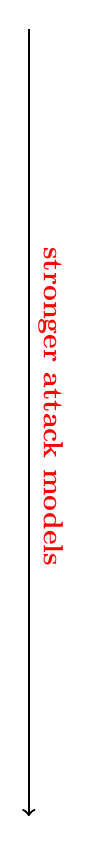
\begin{tikzpicture}[scale=1]
                \node[rotate=270, anchor=south, text=red] at (0,2.2) {\textbf{stronger attack models}};
                \draw[<-, thick, black] (0,-3.0) -- (0,7.0);
            \end{tikzpicture}
        \end{minipage}
    \end{center}

    Come detto in precedenza la \textbf{confidenzialità} in crittografia modeerna equivale a dire che il crittogramma prodotto è \textbf{indistinguibile} da un \textit{random bitstring}. Associando \textbf{IND} ad un modello di attacco andiamo a definire una \textbf{garanzia di sicurezza} dello schema preso in considerazione, ad esempio dire che il nostro schema di crittografia è \textbf{IND-CPA} significa che lo schema è \textbf{indistinguibile da un \textit{random} contro un modello di attacco \textit{Chosen-Plaintext Attack}}.

    \smallskip

    \textcolor{red}{\textbf{IND-EAV (\textit{Indistinguishably under Eavesdropper Attack})}}: è la tipologia di attacco più debole, in quanto un attaccante non sa nulla. Eve è un attaccante passivo che osserva crittogrammi senza eseguire alcuna modifica su di essi e senza interagire con le parti fidate, ma soprattutto senza alcuna conoscenza del testo in chiaro.
\end{flushleft}

\begin{boxA}
    \textcolor{red}{\textbf{\textit{Semantic Security Games on IND-COA}}} \\
    Tutti i \textit{security games} per la confidenzialità sono basati sul concetto di \textbf{indistinguibilità}, un algoritmo eseguito dall'attaccante che ha come scopo di distinguere informazioni dal \textit{plaintext}. 
    
    \smallskip

    Nel modello di attacco \textbf{COA}, l'avversario legge i crittogrammi in transito e prova a indovinare il bit successivo. Riuscirà a vincere il gioco solo se ha un \textit{distinguisher} che indovina il bit corretto con una probabilità $ > 0.5$, nei moderni modelli di attacco, l'avversario non deve necessariamente ottenere la chiave di cifrazione o il contenuto effettivo del testo in chiaro affinché uno schema si consideri ``rotto''.
\end{boxA}

\begin{flushleft}
    \textcolor{red}{\textbf{IND-KPA (\textit{Indistinguishably under Know-Plaintext Attack})}}: Eve è un attaccante passivo che osserva i crittogrammi senza eseguire alcuna modifica su di essi e senza interagire con le parti fidate, ma può conoscere vecchie corrispondenze tra $m$ e $c$ o informazioni sullo spazio dei testi in chiaro, come la distribuzione statistica.
    
    \smallskip

    \textcolor{red}{\textbf{IND-CPA (\textit{Indistinguishably under Chose-Plaintext Attack})}}: è la sicurezza minima richiesta da tutti i moderni crittosistemi, l'attaccante viene modellato per avere accesso ad un \textit{encryption oracle}.

    {\centering
        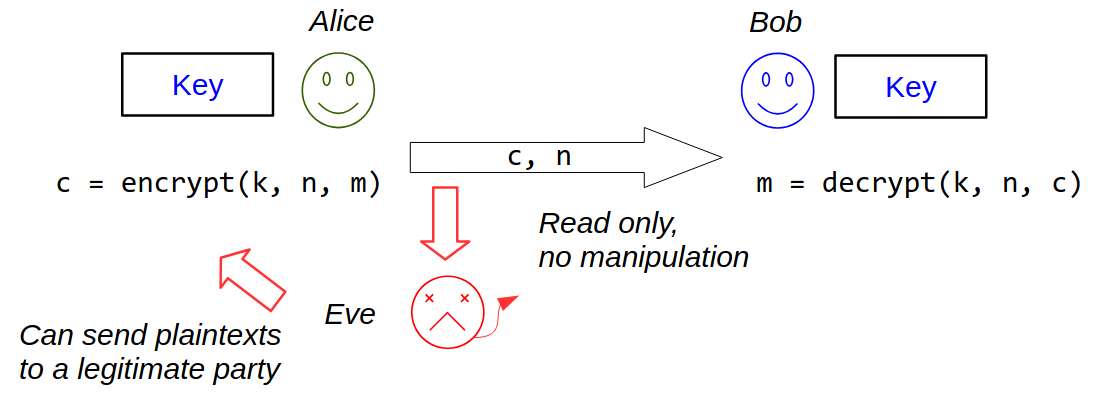
\includegraphics[width=0.45\textwidth]{img/ind_cpa.png}
    \par}

    \textbf{\textit{Security Games}}
    \begin{enumerate}[nosep]
        \item il \textbf{\textit{challenger}} genera una chiave segreta.
        \item l'\textbf{\textit{adversary}} sceglie due messaggi $m_0$ e $m_1$ della stessa lunghezza e gli invia al \textit{challenger}.
        \item il \textit{challenger} genera randomicamente un bit $b \leftarrow \{0, 1\}$ e genera $c = E(m_b)$ e lo invia all'avversario.
        \item l'\textit{adversary} analizza il crittogramma e può scegliere se ripetere gli step dal secondo o passare al quinto.
        \item l'avversario espone come output un valore $b \leftarrow \{0, 1\}$ in base a quale messaggio - se $m_0$ o $m_1$ - è il corrispondente di $c$.
    \end{enumerate}
    L'\textit{adversary} vince il gioco se è capace di riconoscere con una probabilità $ > 0.5\% + negl(l)$ a quale messaggio corrisponde il crittogramma ricevuto.
    
    \smallskip

    Qualunque schema \textbf{deterministico} è intrinsecamente vulnerabile a un attacco del tipo \textbf{IND-CPA}, in quanto basterebbe all'attaccante ripetere lo stesso messaggio per un più iterazioni consecutive e vincere, infatti schemi crittografici sono sicuri sotto la modellazione \textbf{\textit{Distinc Chosen-Plaintext Attack - DCPA}} che obbligano l'\textit{adversary} a scegliere una coppia di messaggi diversi per ogni iterazione del \textit{security game}. Crittografia deterministica è spesso implementata fornendo \textit{nonce} o \textit{IV} fissi (costanti) allo schema, cercando di evitare schemi che sono vulnerabili contro \textit{re-use} di \textit{nonce} o \textit{IV} oppure preferendo schemi che utilizzano \textbf{SIV}. \\
    \textbf{\textit{Deterministic Encryption with Associated Data - DAEAD}} framwork.
\end{flushleft}

\begin{boxA}
    \textcolor{red}{\textbf{IND-CPA e il requisito di impredicibilità dell'IV in CBC}}
    \begin{itemize}[nosep]
        \item \textit{adversary}: sceglie un $m$ che ha lunghezza pari alla \textit{block size} del \textit{block cipher} e lo invia.
        \item \textit{challenger}: sceglie un \textit{IV} e calcola il \textit{ciphertext} $c$, ritornando la coppia $(c, iv)$.
    \end{itemize}
    Facciamo ora un'\textbf{assunzione}: l'avversario conosce l'\textit{IV} successivo - \textbf{\textit{predictable IV}}. \\
    L'avversario può calcolarsi un messaggio $m'$ come $m' = (m \oplus iv \oplus iv')$ dove \textbf{\textit{iv'}} è l'\textit{IV} successivo che utilizzerà il \textit{challenger}. Se il \textit{challenger} cifrerà il messaggio 
    
    {\centering
        $c' = E(iv', m') = E(m' \oplus iv', k) = E(m \oplus \cancel{iv'} \oplus iv \oplus \cancel{iv'}, k) = E(m \oplus iv, k) = c$
    \par}
\end{boxA}

\begin{flushleft}
    \textcolor{red}{\textbf{\textit{IND-CCA1 (Indistinguishably under Chosen-Ciphertext Attack)}}} permette di difendersi contro attacchi attivi sul crittogramma. L'attaccante è capace di manipolare il \textit{ciphertext} al \textit{decryption oracle} (gli input dell'attaccante non sono adattivi per via della definizione data).

    {\centering
        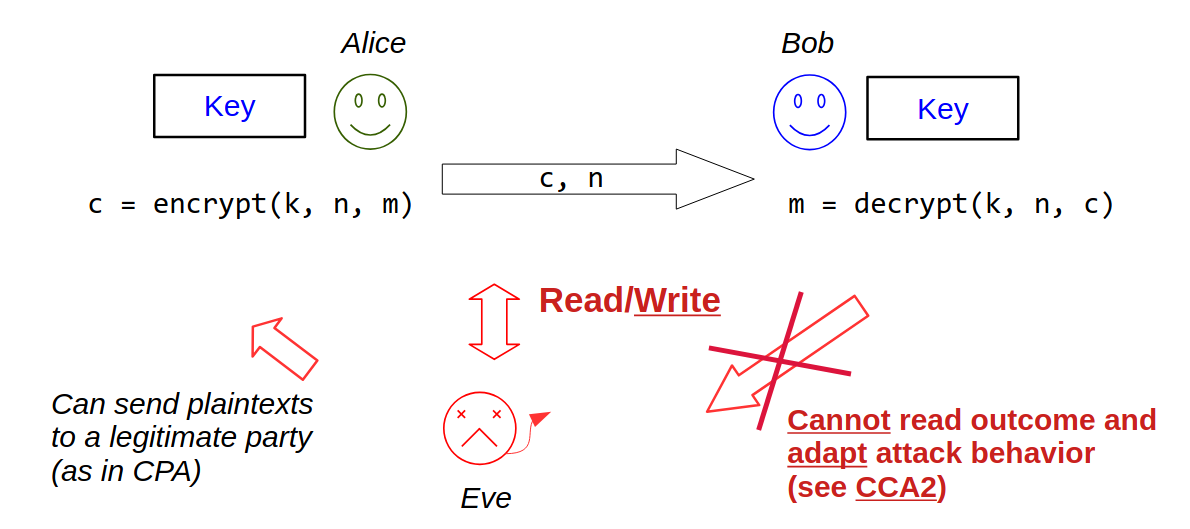
\includegraphics[width=0.45\textwidth]{img/ind_cca1.png}
    \par}

    \textbf{IND-CCA} coinvolge anche \textbf{modifiche al crittogramma} e \textbf{attacchi all'integrità per violare la confidenzialità}. 

    \smallskip

    \textcolor{red}{\textbf{\textit{Malleability}}} si riferisce alla capacità di un'attaccante di ricotruire quali bit del crittogramma sono influenzati dalla modifica di un bit nel testo in chiaro.

    \smallskip

    Un schema crittografico basato su \textcolor{red}{\textbf{\textit{stream cipher}}} viene definito \textbf{\textit{fully malleable}} in quanto una modifica nel testo cifrato in una certa posizione $c_i$ porta ad una modifica nel testo in chiaro nella medesima posizione $p_i$, ad esempio:
    \begin{enumerate}[nosep]
        \item \textit{flipping} il \textbf{bit di direzione} in uno protocollo di comunicazione per eseguire un \textbf{\textit{reflection attack}}.
        \item \textit{flipping} il numero di versione per effettuare un \textbf{\textit{downgrade attack}}.
    \end{enumerate}

    \smallskip

    Per ottenere una certa garanzia di \textbf{integrità} (senza utilizzare \textbf{MAC}) è necessario ricorrere a modalità di crittografia basate su \textit{block cipher}. Andiamo ad osservare il comportamento di uno schema crittografico basato su un qualunque \textit{block cipher} ma che abbia come \textit{mode of operation} \textbf{CBC}, in questo caso analizzando lo schema per decifrare un crittogramma generato, ad esempio, con \textbf{AES-CBC} è fattibile modificare l'\textit{IV}.

    {\centering
        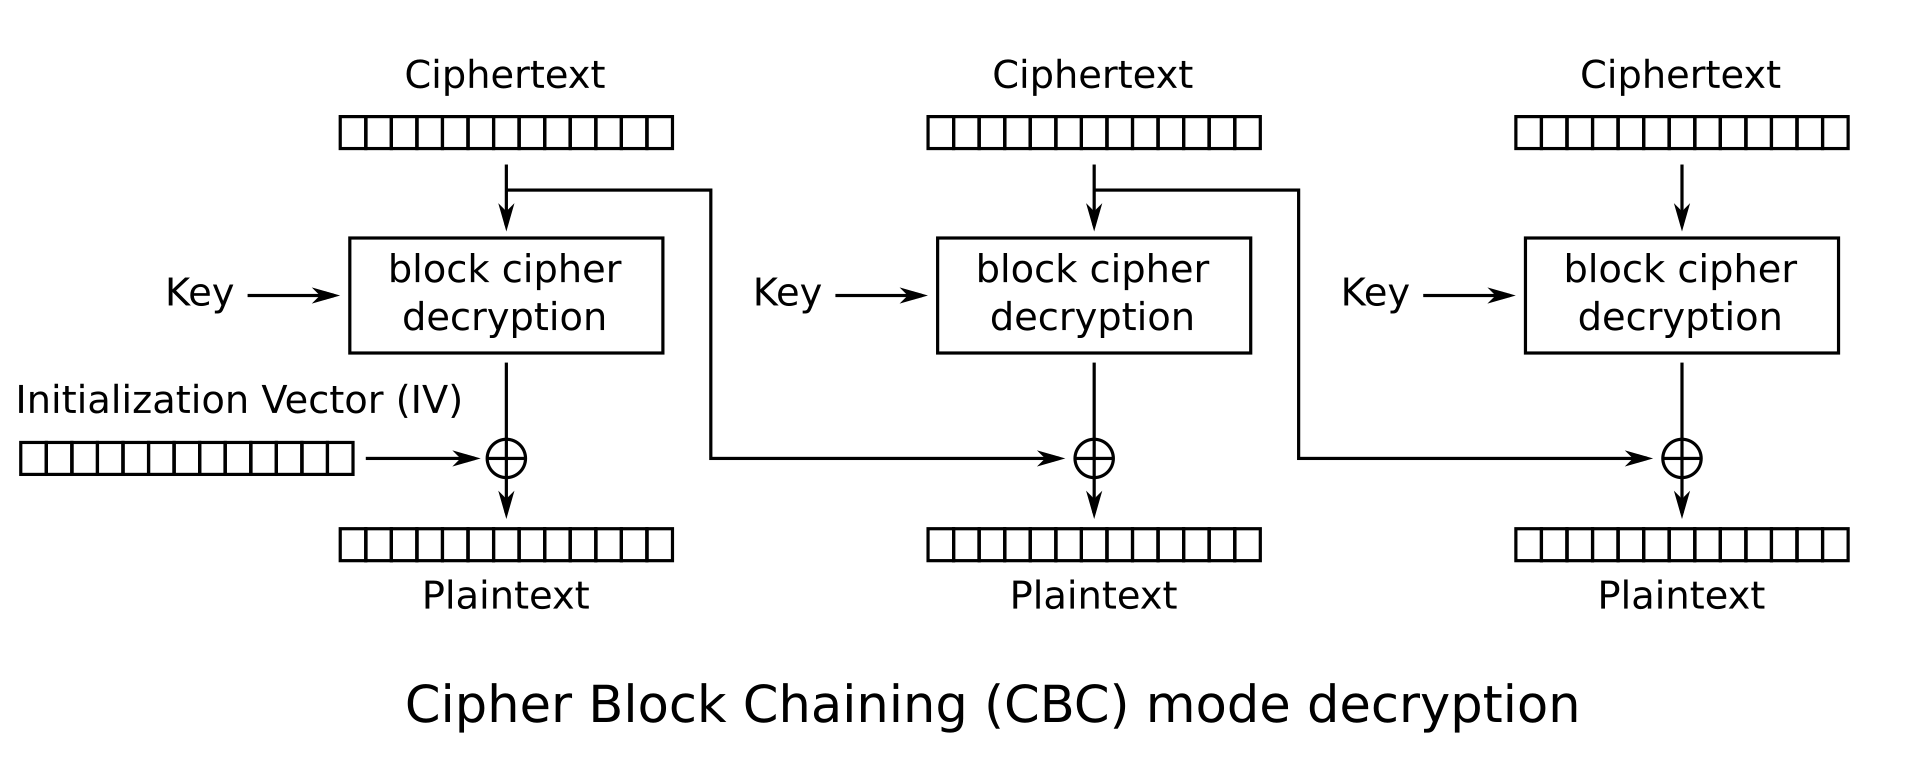
\includegraphics[width=0.45\textwidth]{img/ind_cca1_cbc.png}
    \par}

    Assumiamo che l'attaccante conosca il testo originale $p$ e voglia che in decifrazione venga generato il testo $p'$, nel \textbf{primo blocco}, allora sarebbe possibile calcolarsi un \textit{IV} tale che $IV' = (IV \oplus p \oplus p')$ e sostituire l'\textit{IV} originale con quello generato, in quel caso il primo blocco sarebbe $p'$ e i restanti blocchi rimerrebbero invariati.

    \medskip

    \textcolor{red}{\textbf{\textit{IND-CCA2 (Indistinguishably under Adaptive Chosen-Ciphertext Attack)}}} difende da attacchi attivi iterati e potenzialmente illimitati (l'attaccante è ancora \textbf{polinomiale}), in cui l'attaccante adatta i suoi attacchi in base alla risposta di Bob. L'attaccante invia un testo cifrato manipolato al \textit{decryption oracle}.

    {\centering
        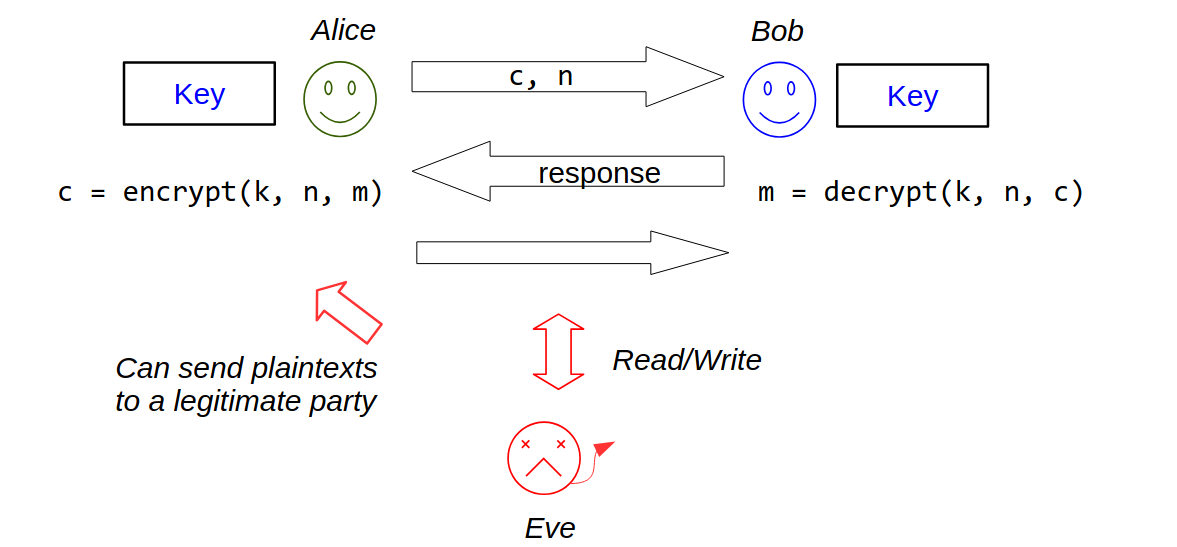
\includegraphics[width=0.45\textwidth]{img/ind_cca2.png}
    \par}
\end{flushleft}

\begin{boxA}
    \textcolor{red}{\textbf{\textit{Padding Oracle Attack}}} \\
    Consideriamo un attacco alle funzioni di \textbf{decifrazione} e \textbf{\textit{unpadding}}, l'attacco ha successo se riusciamo a generare un crittogramma che decifrandolo ha la struttura del \textit{padding} corretto. Gli attacchi al \textit{padding} mirano a manipolare un blocco di un crittogramma $c[i]$ per manipolare il blocco successivo di \textit{plaintext} $p[i+1]$. È simile alla manipolazione dell'\textit{IV} ma in questo caso andiamo a considerare gli ultimi due blocchi del \textit{ciphertext}, modificare il penultimo blocco per manipolare l'ultimo. In questo caso non abbiamo la certezza di come manipolare il crittogramma, ma possiamo \textit{guessare} - questo comporta che, in caso, di un unico tentativo ci siano probabilità trascurabili di successo, se avessimo più tentativi rientraimo nei \textbf{\textit{CCA2 attacks}}.
\end{boxA}

\begin{figure}[h]
    \begin{lstlisting}[mathescape=true]
import string

for character in string.printable:
    c[-2][-1] = character
    p[-1] = c[-2] $\oplus$ D(c[-1])

    if p[-1] has valid padding:
        attack ok
    else:
        attack failed
        \end{lstlisting}
        \label{lst:padding_oracle}
\end{figure}

\begin{boxA}
    Fissiamo \textbf{X} come il \textit{forged ciphertext} e con $\mathbf{X}_n$ l'$n$-simo \textbf{LSB}, \textbf{P} è il \textit{plaintext} originale e \textbf{T} l'output della funzione di decifrazione.
    \begin{enumerate}[nosep]
        \item impostiamo $n=1$ e $\mathbf{X}_n = 0$
        \item eseguiamo la \textit{decryption query} con $D(iv=X, \text{ciphertext}=V)$ e osserviamo la risposta:
        \begin{itemize}[nosep]
            \item \textbf{errore}: il crittogramma decifrato non ha il \textit{padding} valido, quindi $\mathbf{X}_n += 1$ e ripetiamo dal passo 2.
            \item \textbf{ok}: attacco andato a buon fine (tentativi massimo: 256, 128 in media), procediamo al punto 3.
        \end{itemize}
        \item segnamo $\mathbf{X}_n$ come $\mathbf{X}_{n,n}$
        \item se $n=16$ procediamo al passo 5, se no definiamo 
        
        {\centering
            $\mathbf{X}_{m, (m+1)} = [\mathbf{X}_{m,m} \oplus m \oplus (m+1)] \forall \; m \; \in [1, n]$
        \par}
        
        e $n += 1$ e ripetiamo dal passo 2.
        \item in fine possiamo decifrare il \textit{plaintext} originale, nell'ultimo blocco, calcolando:
        
        {\centering
            $P = C \oplus X \oplus [16]$
        \par}

        Dove $[16]$ è un blocco di padding nello standard \textbf{PKCS\#7}
    \end{enumerate}
    Questo attacco funziona perché:
    \begin{itemize}[nosep]
        \item \textbf{V} non viene mai modificato e quindi anche \textbf{T} che è sconosciuto.
        \item la decifratura non modificata esegue: $T \oplus C = P$.
        \item il \textit{padding oracle} ci permette di calcolare \textbf{X} in modo tale che $(T \oplus \mathbf{X}) = [16]$.
        \item $T = (\mathbf{X} \oplus [16])$ e $P = (C \oplus T) = (C \oplus C \oplus [16])$
    \end{itemize}
\end{boxA}

\newpage

\begin{flushleft}
    In questo caso non riuscire a sfruttare la \textbf{malleabilità} del sistema implicherebbe l'impossibilità di effettuare questo tipo di attacco, infatti la probabilità di indovinare il \textbf{padding} di dimensione $n$ sarebbe in media $2^{8n + 1}$ che è \textbf{inefficiente} in $n$. Siccome però in questo caso siamo capaci di sfruttare la malleabilità l'algoritmo abbassa il suo costo a $2^{8 - 1} \cdot n$ tentativi per un padding di dimensione $n$. Per \textbf{AES} sono necessarie all'incirca $\simeq 2000$ iterazioni per decifrare un blocco, è possibile decifrare l'intero crittogramma andando a \textbf{troncare} il crittogramma all'ultimo blocco. 
    
    \smallskip

    In alcuni casi potrebbe essere necessario gestire i falsi positivi del caso 2, al passaggio $n$ potremmo trovare un padding di dimensione $n' > n$
\end{flushleft}

\begin{flushleft}
    \textcolor{red}{\textbf{\textit{Authenticated Encryption}}}: tutti quelli schemi di crittografia che sono resistenti a modelli di attacco \textbf{IND-CCA2} verranno chiamati \textit{authenticated encryption scheme} ovvero schemi che non sono malleabili e che quindi nel caso di modifica, questa verrà rilevata, internamente utilizzano schemi di crittografia insieme a funzioni \textbf{MAC}, alcuni esempi:
    \begin{itemize}[nosep]
        \item \textbf{AES-GCM}: utilizza \textbf{AES-CTR} insieme ad un \textbf{GMAC}.
        \item \textbf{ChaCha20Poly1305}: utilizza \textbf{ChaCha20} insieme ad un autenticatore \textbf{Poly1305}.
        \item \textbf{AES-CCM}: utilizza \textbf{AES-CTR} insieme ad un \textbf{CMAC}.
    \end{itemize}
    Un esempio è quello di \textcolor{red}{\textbf{\textit{EFAIL vulnerability}}}.

    {\centering
        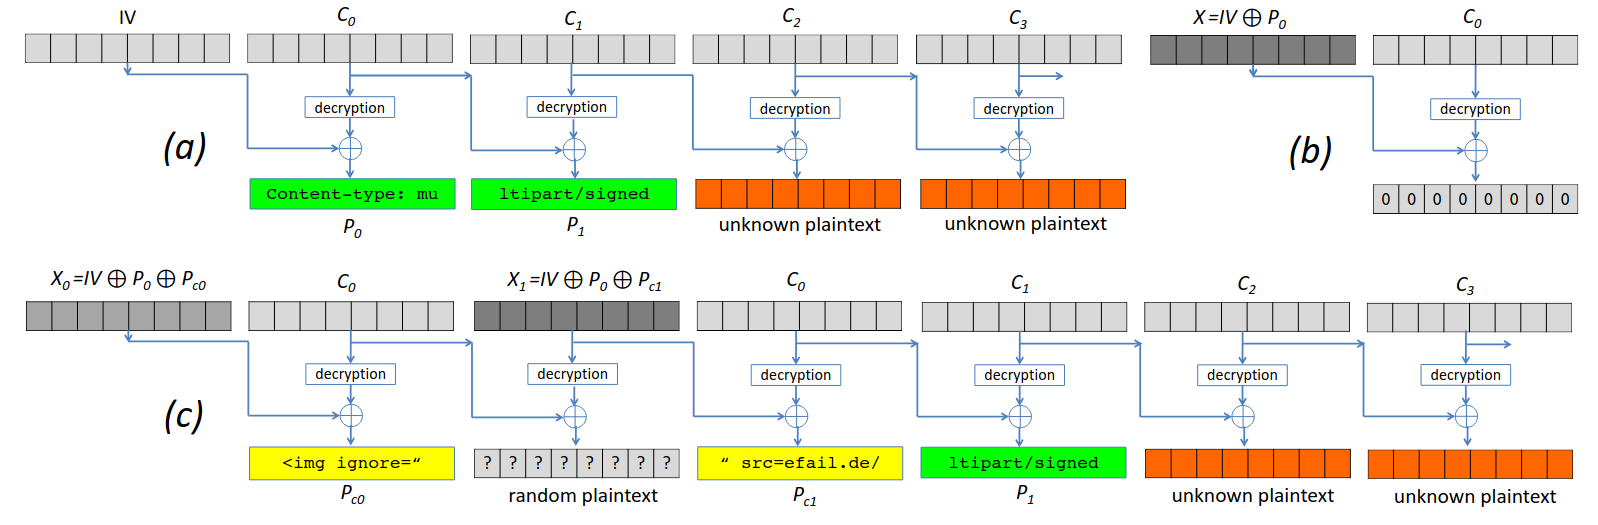
\includegraphics[width=\textwidth]{img/efail.png}
    \par}

    Protocolli crittografici: \textbf{s/MIME} + \textbf{OpenPGP} (\textbf{AES-CBC}), vettore di attacco: \textbf{\textit{Man in the middle}}. L'attaccante esponeva un servizio web che corrispondeva a \textbf{http://efail.de/ltipart/signed} e riuscia a leggere la mail in chiaro all'interno della richiesta.
\end{flushleft}